\documentclass[aspectratio=169]{beamer}

% Theme selection
\usetheme{Madrid}
\usecolortheme{whale}

% Packages
\usepackage[utf8]{inputenc}
\usepackage{amsmath,amssymb,amsfonts}
\usepackage{booktabs}
\usepackage{listings}
\usepackage{tikz}
\usetikzlibrary{shapes.geometric, arrows, positioning}

% Custom Colors
\definecolor{primaryblue}{RGB}{24, 76, 120}
\definecolor{accentcyan}{RGB}{14, 165, 233}
\definecolor{darkgray}{RGB}{30, 41, 59}

\setbeamercolor{palette primary}{bg=primaryblue,fg=white}
\setbeamercolor{titlelike}{parent=palette primary}
\setbeamercolor{block title}{bg=primaryblue,fg=white}
\setbeamercolor{block body}{bg=darkgray!10,fg=black}

% Metadata
\title[Structural Damage VLM Diagnosis]{Structural Damage Image--Text Diagnosis via Qwen3-VL-8B \& LoRA Adaptation}
\subtitle{Controlled 3-Tier Data Bake-Off and Low-VRAM Deployment}
\author[Project Team]{AI Engineering Team}
\institute[Civil AI Lab]{Department of Computer Science \& Civil Engineering}
\date{\today}

\begin{document}

% Slide 1: Title
\begin{frame}
  \titlepage
\end{frame}

% Slide 2: Executive Summary & Objective
\begin{frame}{1. Executive Summary \& Objective}
  \begin{block}{Mission Statement}
    Develop an \textbf{offline, automated multimodal diagnosis pipeline} that takes inspection photos of civil engineering structures (bridges, tunnels, buildings) and produces structured JSON containing both \textbf{multilabel damage categories} and a \textbf{technical morphology description}.
  \end{block}
  \vspace{0.3cm}
  \begin{columns}
    \column{0.48\textwidth}
    \textbf{Target Output JSON Schema:}
    \begin{semiverbatim}\tiny
\{
  "image_id": "00002",
  "damage_categories": ["cracks", "spalling"],
  "description": "Longitudinal fracture running across 
    the reinforced concrete beam with adjacent spalling."
\}
    \end{semiverbatim}
    \column{0.48\textwidth}
    \textbf{Key Project Highlights:}
    \begin{itemize}
      \item \textbf{Backbone:} \texttt{Qwen3-VL-8B-Instruct} (8B VLM).
      \item \textbf{Holdout F1 Score:} \textbf{0.9528} (Multilabel $n=237$).
      \item \textbf{Weighted Metric:} \textbf{0.8268} ($0.6 \text{F1} + 0.4 \text{METEOR}$).
      \item \textbf{Deployment:} Hugging Face LoRA ($\sim 0.7\text{ GB}$).
    \end{itemize}
  \end{columns}
\end{frame}

% Slide 3: Problem Formulation & Challenges
\begin{frame}{2. Problem Formulation \& Domain Challenges}
  \begin{columns}
    \column{0.48\textwidth}
    \begin{alertblock}{Domain Complexities}
      \begin{itemize}
        \item \textbf{Multi-Defect Co-occurrence:} $>64\%$ of images exhibit multiple overlapping defects (e.g. spalling + rebar corrosion).
        \item \textbf{Spatial Orientation Sensitivity:} Descriptions contain critical orientation terms (\textit{"vertical crack"}). Unconstrained image flipping corrupts label alignment!
        \item \textbf{Small Long-Tailed Corpus:} Only $\sim 1,200$ images with rare classes (\textit{honeycomb, efflorescence}).
      \end{itemize}
    \end{alertblock}
    \column{0.48\textwidth}
    \begin{block}{10-Class Closed Taxonomy}
      \begin{enumerate}
        \item \texttt{spalling} \quad 2. \texttt{cracks}
        \item \texttt{corrosion} \quad 4. \texttt{voids}
        \item \texttt{exposed\_rebar} \quad 6. \texttt{peeling}
        \item \texttt{potholes} \quad 8. \texttt{honeycomb}
        \item \texttt{looseness} \quad 10. \texttt{efflorescence}
      \end{enumerate}
    \end{block}
  \end{columns}
\end{frame}

% Slide 4: System Architecture
\begin{frame}{3. End-to-End System Architecture}
  \centering
  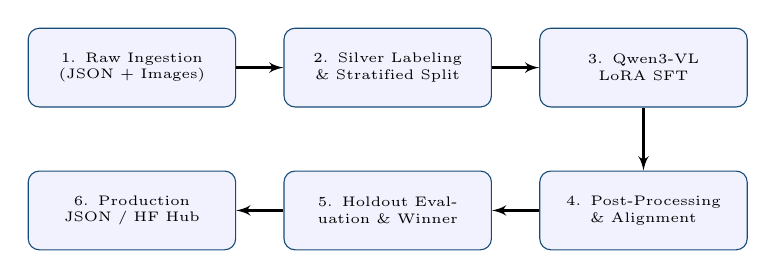
\begin{tikzpicture}[node distance=1.1cm, auto,
    block/.style={rectangle, draw=primaryblue, fill=blue!5, text width=2.4cm, text centered, rounded corners, minimum height=1cm, font=\tiny},
    line/.style={draw, -latex', thick}]
    
    \node [block] (in) {1. Raw Ingestion (JSON + Images)};
    \node [block, right=0.6cm of in] (silver) {2. Silver Labeling \& Stratified Split};
    \node [block, right=0.6cm of silver] (lora) {3. Qwen3-VL LoRA SFT};
    \node [block, below=0.8cm of lora] (post) {4. Post-Processing \& Alignment};
    \node [block, left=0.6cm of post] (eval) {5. Holdout Evaluation \& Winner};
    \node [block, left=0.6cm of eval] (out) {6. Production JSON / HF Hub};
    
    \path [line] (in) -- (silver);
    \path [line] (silver) -- (lora);
    \path [line] (lora) -- (post);
    \path [line] (post) -- (eval);
    \path [line] (eval) -- (out);
  \end{tikzpicture}
  \vspace{0.4cm}
  \begin{itemize}\small
    \item \textbf{Offline-first:} All training, evaluation, and scoring run locally without external cloud dependencies.
    \item \textbf{Unified Post-processing:} Shared deterministic pipeline applied identically to holdout validation and production submission.
  \end{itemize}
\end{frame}

% Slide 5: Data Engineering & Silver Labeling
\begin{frame}{4. Data Engineering \& Stratified Split}
  \begin{columns}
    \column{0.48\textwidth}
    \begin{block}{Silver Label Synthesis Formula}
      Due to uncurated raw annotations, silver multi-labels $L_i$ are synthesized via:
      $$L_i = \text{Prefix\_Seeds}(\text{filename}_i) \cup \text{Keywords}(\text{description}_i)$$
      \begin{itemize}\footnotesize
        \item \textbf{Prefix Seeds:} e.g. \texttt{crack\_} $\to$ \texttt{cracks}, \texttt{gangf\_} $\to$ \texttt{exposed\_rebar} + \texttt{cracks}.
        \item \textbf{Longest-First Match:} Matches multi-word synonyms first to prevent subword false alarms.
      \end{itemize}
    \end{block}
    \column{0.48\textwidth}
    \begin{block}{Frozen Multi-Label Stratification}
      \begin{itemize}\footnotesize
        \item \textbf{Algorithm:} \texttt{MultilabelStratifiedShuffleSplit} ($80/20$, seed $42$).
        \item \textbf{Train Set:} $963$ samples.
        \item \textbf{Holdout Val Set:} $237$ samples.
        \item \textbf{Artifact:} \texttt{data/processed/splits/v1.json}.
        \item \textbf{Guarantee:} Zero validation leakage across all comparative experiments.
      \end{itemize}
    \end{block}
  \end{columns}
\end{frame}

% Slide 6: Three-Tier Data Bake-Off
\begin{frame}{5. Three-Tier Data Augmentation Bake-Off}
  \begin{table}[h]\small
    \centering
    \begin{tabular}{lp{3.5cm}p{3.5cm}p{3.5cm}}
      \toprule
      \textbf{Parameter} & \textbf{Tier A (Baseline SFT)} & \textbf{Tier B (Orientation-Safe)} & \textbf{Tier C (Hybrid Expansion)} \\
      \midrule
      \textbf{Dataset Size} & $963$ clean pairs & $1,926$ pairs (Orig + Aug) & $2,889+$ expanded pairs \\
      \textbf{Image Augmentation} & None ($0$ distortion) & Photometric (blur, noise) + Conditional Geometric & None \\
      \textbf{Orientation Rule} & Preserved naturally & \textbf{Flip strictly forbidden} if direction text present & Preserved naturally \\
      \textbf{Text Expansion} & Longest raw description & Normalized technical sentences & Local Paraphrase $\times 3$ + Pseudo-captioning \\
      \bottomrule
    \end{tabular}
  \end{table}
\end{frame}

% Slide 7: VRAM-Safe LoRA Recipe
\begin{frame}{6. VRAM-Safe LoRA Training Recipe}
  \begin{columns}
    \column{0.52\textwidth}
    \begin{block}{Hyperparameters (LLaMA-Factory)}
      \begin{itemize}\footnotesize
        \item \textbf{PEFT Method:} LoRA ($\text{Rank } r = 64, \alpha = 128$).
        \item \textbf{Target Modules:} \texttt{q, k, v, o, gate, up, down\_proj}.
        \item \textbf{Vision Tower:} \textbf{Frozen} (saves $\sim 18\text{ GB}$ VRAM).
        \item \textbf{Effective Batch Size:} $1 \times 16 = 16$.
        \item \textbf{Precision \& LR:} BF16, $\text{LR} = 1.0 \times 10^{-4}$ (Cosine).
        \item \textbf{Max Resolution:} $524,288$ pixels ($\sim 0.5\text{ MP}$).
      \end{itemize}
    \end{block}
    \column{0.44\textwidth}
    \begin{block}{Resource Footprint (Ada 49GB)}
      \begin{itemize}\footnotesize
        \item \textbf{Peak Memory:} $\sim 28.5\text{ GB} / 49.0\text{ GB}$.
        \item \textbf{Training Time:} $< 45$ minutes ($3$ epochs).
        \item \textbf{Loss Convergence:} Smooth decline from $1.82 \to 0.249$.
      \end{itemize}
    \end{block}
  \end{columns}
\end{frame}

% Slide 8: Post-Processing Pipeline
\begin{frame}{7. Deterministic Post-Processing \& Alignment}
  \begin{block}{Four-Stage Reliability Stack}
    \begin{enumerate}\small
      \item \textbf{JSON Repair:} Strips conversational preambles and markdown fences (\texttt{```json}).
      \item \textbf{Synonym Mapping:} Canonicalizes all free-form damage strings into the closed 10-class set.
      \item \textbf{Bidirectional Text-Category Sync:} Injects standardized morphology sentences when a category is listed but omitted from the description text.
      \item \textbf{Sentence Deduplication:} Removes redundant phrases and normalizes whitespace.
    \end{enumerate}
  \end{block}
\end{frame}

% Slide 9: Results & Winner Selection
\begin{frame}{8. Holdout Evaluation \& Winner Selection}
  \begin{table}[h]\small
    \centering
    \begin{tabular}{lccccc}
      \toprule
      \textbf{Tier} & \textbf{Multilabel F1} & \textbf{METEOR} & \textbf{Weighted Score} & \textbf{Safety Gate} & \textbf{Rank} \\
      \midrule
      \textbf{Tier A (Clean)} & \textbf{0.9528} & 0.6379 & \textbf{0.82684} & \textbf{Pass (Baseline)} & \textbf{1 (Winner)} \\
      \textbf{Tier B (Aug)} & 0.9495 & \textbf{0.6427} & 0.82681 & Pass ($\ge 0.9242$) & 2 \\
      \textbf{Tier C (Hybrid)} & 0.9378 & 0.6136 & 0.80814 & Pass ($\ge 0.9242$) & 3 \\
      \bottomrule
    \end{tabular}
  \end{table}
  \vspace{0.2cm}
  \begin{block}{Winner Decision Rule}
    $$\text{Score} = 0.6 \times \text{F1} + 0.4 \times \text{METEOR}, \quad \text{subject to } \text{F1} \ge 0.97 \times \max(\text{F1})$$
    \textbf{Insight:} Tier A achieved the highest classification precision with zero hallucinated noise.
  \end{block}
\end{frame}

% Slide 10: Production Retraining & Deployment
\begin{frame}{9. Production Retraining \& Low-VRAM Deployment}
  \begin{columns}
    \column{0.48\textwidth}
    \begin{block}{Full Retrain on data\_v2}
      \begin{itemize}\small
        \item Retrained on all $1,200$ images using the winning Tier A recipe.
        \item Final training loss: $\mathbf{0.249}$.
        \item Output adapter: \texttt{outputs/runs/full\_winner\_v2}.
      \end{itemize}
    \end{block}
    \column{0.48\textwidth}
    \begin{block}{Hugging Face \& Low-VRAM}
      \begin{itemize}\small
        \item \textbf{Repo:} \texttt{nhantran214/damage-vlm-qwen3vl-8b-lora}
        \item \textbf{Full Precision (BF16):} $\sim 18\text{ GB}$ VRAM.
        \item \textbf{4-Bit NF4 (\texttt{bitsandbytes}):} $\sim \mathbf{5.8\text{ GB}}$ VRAM (runs on RTX 3060/4060).
      \end{itemize}
    \end{block}
  \end{columns}
\end{frame}

% Slide 11: Conclusion
\begin{frame}{10. Conclusion \& Future Directions}
  \begin{block}{Key Contributions}
    \begin{itemize}\small
      \item \textbf{Methodology:} Established that clean SFT outperforms noisy augmentation for civil structure diagnosis.
      \item \textbf{Performance:} Achieved $0.9528$ F1 score with 100\% valid JSON compliance.
      \item \textbf{Accessibility:} Published lightweight LoRA adapter deployable on $6\text{ GB}$ consumer GPUs.
    \end{itemize}
  \end{block}
  \vspace{0.2cm}
  \begin{block}{Future Extensions}
    \begin{itemize}\small
      \item High-capacity offline local LLM paraphrasing (e.g. Qwen2.5-14B).
      \item Unfreezing vision projector for sub-millimeter micro-crack detection.
      \item Bounding-box defect localization with calibrated confidence scoring.
    \end{itemize}
  \end{block}
\end{frame}

\end{document}
